\documentclass[journal]{IEEEtran}
\usepackage[pdftex]{graphicx}
\usepackage[cmex10]{amsmath}
\usepackage{ifthen}
\usepackage{stfloats}

% declare the path(s) where your graphic files are
\graphicspath{{./diagrams/}}

\begin{document}

% paper title
% can use linebreaks \\ within to get better formatting as desired
\title{Dynamic Load Balancing for\\Heterogeneous Systems}

% author names and IEEE memberships
\author{Kenneth~Lee,~Kyle~Morgan}%

% The paper headers
\markboth{CS 5504: Computer Architecture}{Final Project Paper, 5 December 2011}

% make the title area
\maketitle

\begin{abstract}
Leveraging maximimum performance from specialized hardware is one of the
major problems facing computer scientists today.  General-purpose computing
on graphics processing units (GPGPU) is a technique that is becoming
increasingly popular for handling computations typically performed by the
CPU.  However, many GPGPU algorithms place the entire workload on the Graphics
processing unit (GPU) leaving the CPU idle for the duration of the computation.
This paper investigates the effect various load-balancing schemes across the CPU
and GPU have on overall application performance.  Additionally, the discrete and
fused GPU architectures, and their impact on performance, will be investigated.
\end{abstract}

\section{Introduction}
% The very first letter is a 2 line initial drop letter followed
% by the rest of the first word in caps.
% 
% form to use if the first word consists of a single letter:
% \IEEEPARstart{A}{demo} file is ....
% 
% form to use if you need the single drop letter followed by
% normal text (unknown if ever used by IEEE):
% \IEEEPARstart{A}{}demo file is ....
% 
% Some journals put the first two words in caps:
% \IEEEPARstart{T}{his demo} file is ....
\IEEEPARstart{L}{everaging} the maximum performance from specialized hardware is one
of the major problems facing computer scientists today.  The unique architecture of the
GPU gives it a place as a massively parallel hardware accelerator.  Programming frameworks
such as OpenCL allow programmers to utilize the stream processors of the GPU for non-graphics
data.  However, because of the difficulty in programming for this hardware, most of the
effort is spent on trying to achieve performance from the GPU, while the CPU is left
unused.  By also making use of CPU to process a chunk of the data, we can achieve higher
utilization of resources and therefore increase overall program performance.

GPU+CPU co-processing hardly a new idea.  Jimenez et al.~\cite{Jimenez2009} present a
dynamic library which can be used in a system to dynamically schedule tasks for GPU
computation across various processes. The method described only looks at optimizing
usage of the GPU across the whole system, rather than optimizing a single application’s
performance. The StarPU system, on the other hand, presents a method of co-processing
and load balancing on a per application basis~\cite{Augonnet2009}. They show that by
using an appropriate model for the load balancing, they are able to achieve improvements
in speed for applications which call for code acceleration multiple times.  We intend
to extend this work to improve the speed of each kernel execution by splitting the
work of that kernel over the capable resources, similar to the schemes used by
OpenMP~\cite{Dagum1998}. Both of these papers address data transfer times as a major cost
of GPU computing. Using the new AMD Fusion architecture, which fuses the CPU and GPU onto
a single die, we may be able to eliminate or greatly reduce this cost, which will impact
the overhead of GPU+CPU co-processing.

We expect that by using GPU+CPU processing we will improve the performance of the
application, when compared to CPU-only or GPU-only.  That is, consider a workload of size
$n$, a GPU that requires $t_g$ time to perform one block of computation, and a CPU that
requires $t_c$ time to perform one block of computation. We expect that the GPU would
require time $nt_g$ to perform a given computation, while the CPU would require $nt_c$
time to perform the same computation.  Optimally, we would expect the load-balancing
scheme to require the following time to perform the computation.
\[\max{\{(n-m)t_g, mt_c}\} + t_d + t_o\]
Where $m$ is the amount of the workload given to the CPU ($m \leq n$), $t_d$ is the data
transfer cost, and $t_o$ is any overhead incurrent from synchronization costs of the load
balancing scheme or otherwise.  The above will be faster than just the GPU iff
$t_g - \max{\{(n-m)t_g, mt_c}\} < t_d + t_o$.

Two different load balancing schemes were implemented for this paper.  The first was a
static load balancer, which partitions the workload in two, and transfers one chunk to
the CPU, and the other to the GPU.  The CPU and GPU work entirely independently, and
their results are merged once each finish.  The static load balancer should have no
synchronization overhead, and transfers all of the data prior to the computation.
The main caveat with a static load balancer is that the ratio of the workload given to
the CPU is chosen by the load balancer.  An optimal ratio would be one such that the
time to perform the computation is equal for both the CPU and GPU.  Unfortunately, this
optimal ratio will be application-dependent, meaning that a fixed ratio cannot be optimal
for every application.  In order for a static load balancer to be optimal for a given
application, a programmer must tune the amount of workload given to the CPU that works
best for that application.

The second scheme is a dynamic load balancer, which partitions the data into many smaller
chunks.  One chunk is sent to the CPU and GPU each for computation.  When one finished,
it requests another chunk from the load balancer, and this process repeats until the
entirely workload has been sent to either the CPU or GPU.  The dynamic load balancer
will incur some amount of synchronization overhead, because shared variables that track
which chunks of the workload are left must be protected by a lock.  Unlike the static
load balancer, the dynamic load balancer transfers data throughout the computation.
The dynamic load balancer is designed to mitigate the primary problem with the static
load balancer - that the optimal ratio of computation performed on the CPU is
application-dependent.  A chunk size must be chosen such that the processing units are
not requesting chunks so frequently that contention for shared variables rise and
synchronization overhead increases, yet small enough to not allow one processing unit
to receive a disproportionate amount of work.

\section{Architecture Overview}
In this section we discuss the different architectures of the experimental
machines under test.  We will discuss CPU, GPU, and APU architectures in
terms of major differences that affect the performance of the device.  

\subsection{CPU Architecture}
The CPU architecture is designed as a low latency architecture.  To facilitate
the needs for low latency application performance, a series of hierarchical 
caches have been designed to hide memory access costs, the most common cause
of latency in single-threaded applications on modern architectures.  Each core
of the CPU typically only runs one or two hardware-enabled threads to reduce
cache pollution, thus avoiding latency.  An example CPU architecture is given
by Figure~\ref{fig:cpu_arch}.

The use of the Single Instruction Multiple Data (SIMD) paradigm enables increased
performance on these devices by increasing data throughput for data parallel
applications.

\subsection{GPU Architecture}
The GPU almost acts a foil to the CPU architecture.  Instead of optimizing the
architecture of the device to increase performance of a single thread, the GPU
architecture is specifically designed for large throughput performance.  

The memory hierarchy for the GPU architecture is given by Figure~\ref{fig:gpu_arch}.

\begin{figure}[t]
\centering
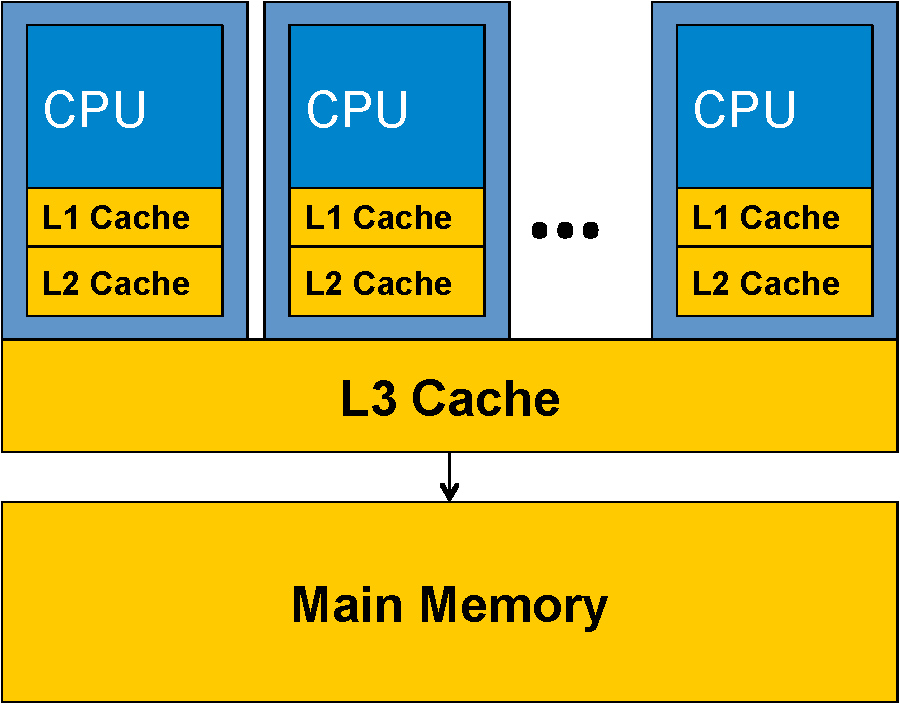
\includegraphics[width=2.5in]{cpu_architecture}
\caption{CPU Architecture}
\label{fig:cpu_arch}
\end{figure}

\begin{figure}[t]
\centering
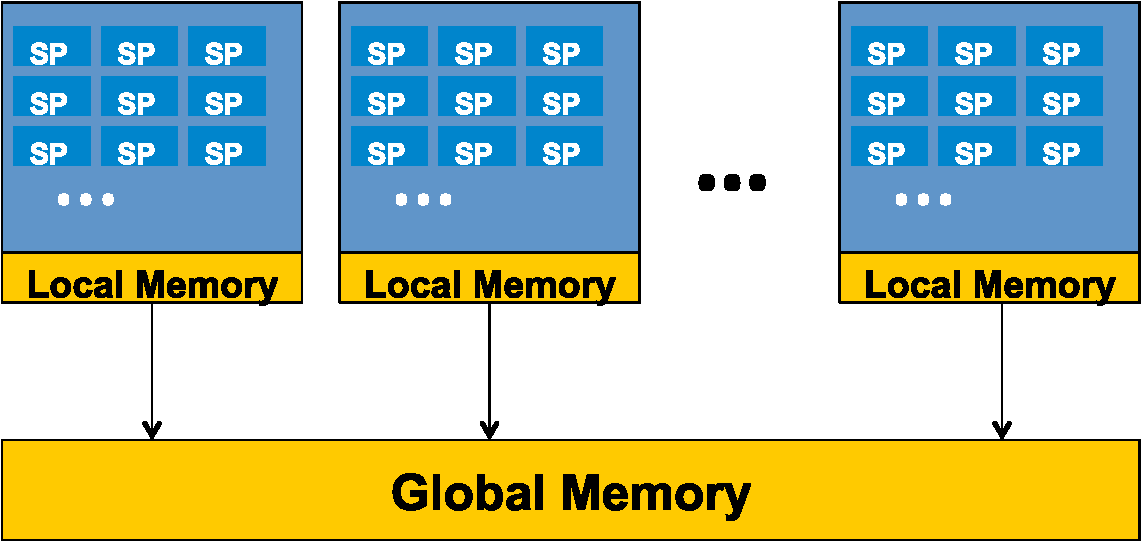
\includegraphics[width=2.5in]{gpu_architecture}
\caption{GPU Architecture}
\label{fig:gpu_arch}
\end{figure}

\subsection{APU Architecture}
The APU is a relatively new, novel architecture that attempts to 
improve on the the discrete CPU+GPU system.  The CPU die is split
between the typical CPU processor as well as allocating space
for a SIMD engine, the basis for a GPU processor.  The APU has a 
shared memory between the CPU and SIMD engine, in which accesses
are facilitated through a high-speed memory controller.  The AMD
Fusion technology is an example of this type of architecture~\cite{AMDFusion}.

One of the main benefits of the APU is the elimination of the PCI-e
bus, which allows for much faster transfer between CPU and GPU.  Daga et al.
show that the AMD Fusion architecture allows for much faster data transfers
between CPU and GPU, allowing for an overall improvement in runtime, despite
reduced compute power on the GPU~\cite{Daga2011}. 

\section{Load Balancing Benchmarks}

For this paper, three different benchmarks were used to assess the
effectiveness of the load balancer.  The first is a reduction benchmark,
in which the sum of variably-sized array is computed.  The reduction benchmark
is unique in that different code is being run on the CPU and the GPU.  The
reason for this is that the GPU cannot efficiently compute a reduction the way
a CPU typically would -- due to the relative innefficiency of backward branches
on the GPU.  A reduction on the GPU is a multi-stage process, in which the
output of one step is used as the input of the next.  Each steam processor
computes the reduction of two elements during each iteration, reducing the amount
of work during each step by a factor of two.  As a result, each step utilizes half
the stream processors of the previous step.  This continues until the reduction
operation is only done by a single stream processor.  A natural consequence of
this algorithm is that not all of the stream processors will be utilized during
the computation.

The next benchmark is a simple vector addition operation that computes the sum
of two input vectors, and stores the result into an output vector.  The third
benchmark, referred henceforth as the ``Vector Add+'' benchmark, is similar to
the Vector Add benchmark, but it computes 1000 additions before storing the result
in the output vector.  The motivation behind this benchmark is to reduce memory
access overhead with more computation.

\section{Results}
\begin{figure}[t]
\centering
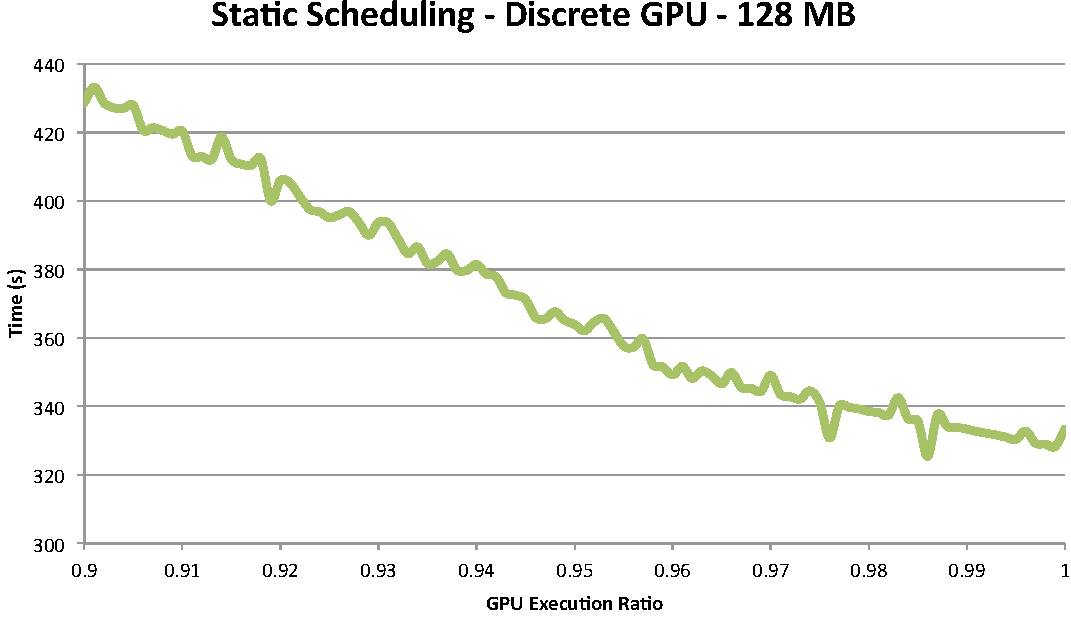
\includegraphics[width=3.0in]{static_discrete}
\caption{Varying Data Ratio with a Discrete GPU}
\label{fig:static_discrete}
\end{figure}

Consider Figure \ref{fig:static_discrete}, where the amount of data
executed on the GPU is varied between 90\% and 100\%.  The total execution
time including data transfers has an obvious downward trend as more
data is executed on the GPU.  However, there are a couple of static
ratios which yielded better performance than executing all of the data
on the GPU.  Most notably, when only 98.6\% of the data was executed on
the GPU.  In this instance, the overall execution time was 325.27 seconds,
compared to 333.31 seconds with only the GPU -- a ~2.4\% speedup.

\begin{figure}[t]
\centering
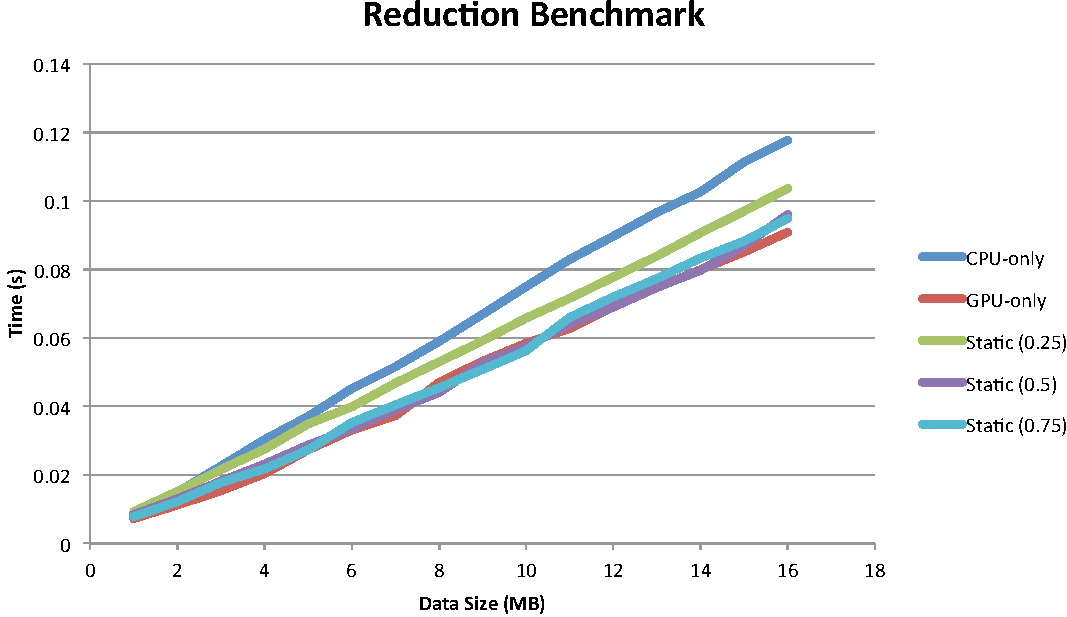
\includegraphics[width=3.0in]{reduce_fused}
\caption{Reduction Benchmark on an APU Architecture}
\label{fig:reduce_fused}
\end{figure}

\begin{figure}[t]
\centering
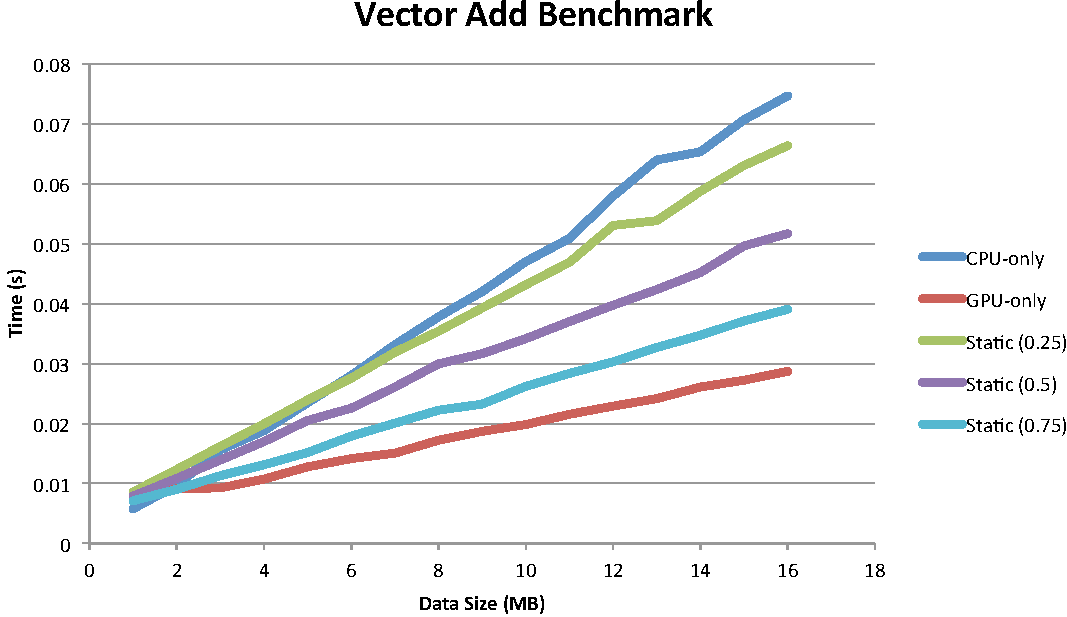
\includegraphics[width=3.0in]{vector_fused}
\caption{Vector Add Benchmark on an APU Architecture}
\label{fig:vector_fused}
\end{figure}

\begin{figure}[t]
\centering
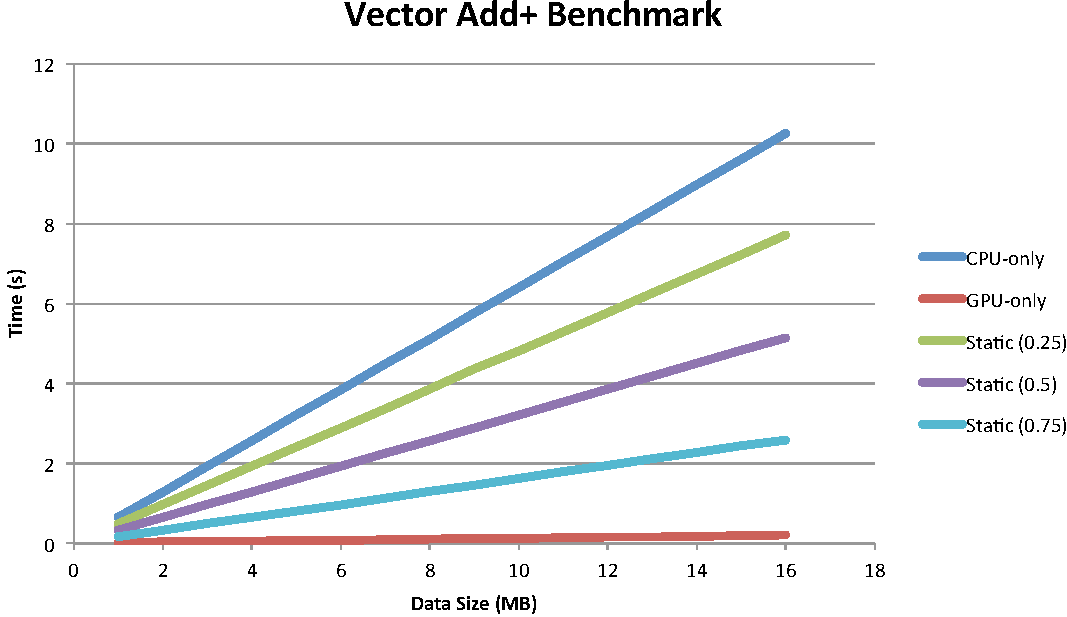
\includegraphics[width=3.0in]{vector_plus_fused}
\caption{Vector Add+ Benchmark on an APU Architecture}
\label{fig:vector_plus_fused}
\end{figure}

Next, consider Figures \ref{fig:reduce_fused}, \ref{fig:vector_fused}, and
\ref{fig:vector_plus_fused}. The figures demonstrate a variety of different
load balancing options for the Reduction, Vector Add, and Vector Add+
benchmarks, across data sizes ranging between 1 MB and 16 MB.  Each figure
depicts the total execution time for the CPU-only and GPU-only computations,
as well as static load balancing with 25\%, 50\%, and 75\% of the data on the
GPU.  In each of the figures, it's evident that the GPU performs significantly
faster than the CPU for the given benchmarks, with the static partitioning
schemes lying somewhere between the two.

\section{Analysis}
Lorem ipsum dolor sit amet, consectetur adipisicing elit, sed do
eiusmod tempor incididunt ut labore et dolore magna aliqua. Ut
enim ad minim veniam, quis nostrud exercitation ullamco laboris
nisi ut aliquip ex ea commodo consequat. Duis aute irure dolor
in reprehenderit in voluptate velit esse cillum dolore eu fugiat
nulla pariatur. Excepteur sint occaecat cupidatat non proident,
sunt in culpa qui officia deserunt mollit anim id est laborum.

\section{Related Work}
Ryoo et al. discuss optimization strategies for GPU versus CPU runtime
systems~\cite{Ryoo2007}.  However, their research is based on a GPU-only
or CPU-only implementation instead of a heterogeneous approach.  The work
presented in ~\cite{Jablin2011} describes a runtime and compiled framework
for improving memory access latency and reducing data transfer overhead
for GPU kernels.  Our work differs from this, because the kernel execution
was still being performed soley on the GPU, whereas our work investigates
kernel execution on multiple devices.

Computation via heterogeneous systems is a relatively new research area for
high performance computing.  The various frameworks and large number of
different accelerator devices can make this quite difficult for application
programmers to manage.  The StarPU system~\cite{Augonnet2009} presents a 
framework to allow for programmers to write numerical codelets and have them
automatically run on a heterogeneous system.  Scheduling work for this system
is one of the most difficult parts of the system, because of the various
overheads for work-sharing schemes. We simplify this work, by looking at a
two-device system, and focus on the performance characteristics of different
scheduling scheme.  Verner et al. use this approach to create a high-throughput
low-lantecy heterogeneous encryption system~\cite{Verner2011}. 

Jimenez et al.~\cite{Jimenez2009} present a dynamic library which can be used
in a system to dynamically schedule tasks for GPU computation across various
processes. The method describes only looks at optimizing usage of the GPU across
the whole system, instead of optimizing a single application's performance.

% An example of a floating figure using the graphicx package.
% Note that \label must occur AFTER (or within) \caption.
% For figures, \caption should occur after the \includegraphics.
% Note that IEEEtran v1.7 and later has special internal code that
% is designed to preserve the operation of \label within \caption
% even when the captionsoff option is in effect. However, because
% of issues like this, it may be the safest practice to put all your
% \label just after \caption rather than within \caption{}.
%
% Reminder: the "draftcls" or "draftclsnofoot", not "draft", class
% option should be used if it is desired that the figures are to be
% displayed while in draft mode.
%
%\begin{figure}[!t]
%\centering
%\includegraphics[width=2.5in]{myfigure}
% where an .eps filename suffix will be assumed under latex, 
% and a .pdf suffix will be assumed for pdflatex; or what has been declared
% via \DeclareGraphicsExtensions.
%\caption{Simulation Results}
%\label{fig_sim}
%\end{figure}

% Note that IEEE typically puts floats only at the top, even when this
% results in a large percentage of a column being occupied by floats.


% An example of a double column floating figure using two subfigures.
% (The subfig.sty package must be loaded for this to work.)
% The subfigure \label commands are set within each subfloat command, the
% \label for the overall figure must come after \caption.
% \hfil must be used as a separator to get equal spacing.
% The subfigure.sty package works much the same way, except \subfigure is
% used instead of \subfloat.
%
%\begin{figure*}[!t]
%\centerline{\subfloat[Case I]\includegraphics[width=2.5in]{subfigcase1}%
%\label{fig_first_case}}
%\hfil
%\subfloat[Case II]{\includegraphics[width=2.5in]{subfigcase2}%
%\label{fig_second_case}}}
%\caption{Simulation results}
%\label{fig_sim}
%\end{figure*}
%
% Note that often IEEE papers with subfigures do not employ subfigure
% captions (using the optional argument to \subfloat), but instead will
% reference/describe all of them (a), (b), etc., within the main caption.


% An example of a floating table. Note that, for IEEE style tables, the 
% \caption command should come BEFORE the table. Table text will default to
% \footnotesize as IEEE normally uses this smaller font for tables.
% The \label must come after \caption as always.
%
%\begin{table}[!t]
%% increase table row spacing, adjust to taste
%\renewcommand{\arraystretch}{1.3}
% if using array.sty, it might be a good idea to tweak the value of
% \extrarowheight as needed to properly center the text within the cells
%\caption{An Example of a Table}
%\label{table_example}
%\centering
%% Some packages, such as MDW tools, offer better commands for making tables
%% than the plain LaTeX2e tabular which is used here.
%\begin{tabular}{|c||c|}
%\hline
%One & Two\\
%\hline
%Three & Four\\
%\hline
%\end{tabular}
%\end{table}


% Note that IEEE does not put floats in the very first column - or typically
% anywhere on the first page for that matter. Also, in-text middle ("here")
% positioning is not used. Most IEEE journals use top floats exclusively.
% Note that, LaTeX2e, unlike IEEE journals, places footnotes above bottom
% floats. This can be corrected via the \fnbelowfloat command of the
% stfloats package.



\section{Conclusion}
Lorem ipsum dolor sit amet, consectetur adipisicing elit, sed do
eiusmod tempor incididunt ut labore et dolore magna aliqua. Ut
enim ad minim veniam, quis nostrud exercitation ullamco laboris
nisi ut aliquip ex ea commodo consequat. Duis aute irure dolor
in reprehenderit in voluptate velit esse cillum dolore eu fugiat
nulla pariatur. Excepteur sint occaecat cupidatat non proident,
sunt in culpa qui officia deserunt mollit anim id est laborum.

\begin{thebibliography}{1}

\bibitem{Augonnet2009}
C.~Augonnet, S.~Thibault, R.~Namyst, and P.A.~Wacrenier,
``StarPU: A Unified Platform for Task Scheduling on Heterogeneous Multicore Architectures'' in
\emph{Proceedings of the 15th International Euro-Par Conference on Parallel Processing}, 2009, pp. 863-874.

\bibitem{Che2009}
S.~Che, M.~Boyer, J.~Meng, D.~Tarjan, J.W.~Sheaffer, S.H.~Lee, and K.~Skadron,
``Rodinia: A benchmark suite for heterogeneous computing'' in
\emph{Proceedings of the 2009 IEEE International Symposium on Workload Characterization (IISWC)}, 2009, pp. 44-54.

\bibitem{Daga2011}
M.~Daga, A.M.~Aji, and W.~Feng,
``On the Efficacy of a Fused CPU+GPU Processor (or APU) for Parallel Computing'' in
\emph{Application Accelerators in High-Performance Computing (SAAHPC)}, 2011, pp. 141-149.

\bibitem{Dagum1998}
L.~Dagum and R.~Menon,
``OpenMP: An industry-standard API for shared-memory programming'' in
\emph{IEEE Computational Science and Engineering} 1998, pp. 46–55.

\bibitem{Danalis2010}
A.~Danalis, G.~Marin, C.~McCurdy, J.S.~Meredith, P.C.~Roth, K.~Spafford, V.~Tipparaju, and J.S.~Vetter,
``The Scalable Heterogeneous Computing (SHOC) benchmark suite'' in
\emph{Proceedings of the 3rd Workshop on General-Purpose Computation on Graphics Processing Units}, 2010, pp. 63-74.

\bibitem{Jablin2011}
J.A.~Jablin, P.~McCormick, and M.~Herlihy,
``Scout: High-Performance Heterogeneous Computing Made Simple'' in
\emph{Parallel and Distributed Processing Workshops and Phd Forum (IPDPSW)}, 2011, pp. 2093-2096.

\bibitem{Jimenez2009}
V.J.~Jiménez, L.~Villanova, I.~Gelado, M.~Gil, G.~Fursin, and N.~Navarro,
``Predictive Runtime Code Scheduling for Heterogeneous Architectures'' in
\emph{Proceedings of the 4th International Conference on High Performance Embedded Architectures and Compilers}, 2009, pp. 19-33.

\bibitem{Ryoo2007}
S.~Ryoo, C.I.~Rodrigues, S.S.~Baghsorkhi, S.S.~Stone, D.B.~Kirk, and W.W.~Hwu,
``Optimization Principles and Application Performance Evaluation of a Multithreaded GPU Using CUDA'' in
\emph{Proceedings of the 13th ACM SIGPLAN Symposium on Principles and practice of parallel programming}, 2007, pp. 73-82.

\bibitem{Verner2011}
U.~Verner, A.~Schuster, and M.~Silberstein,
``Processing data streams with hard real-time constraints on heterogeneous systems'' in
\emph{Proceedings of the international conference on Supercomputing}, 2011, pp. 120-130.

\end{thebibliography}

\setboolean{@twocolumn}{false}
\newpage
\appendix[Team Member Contributions]
Kenneth Lee did A, B, C.  Kyle Morgan did X, Y, Z.
\end{document}
